% ============================================================================
% Supplementary Figures
% Shared between Supplementary.tex (standalone) and main_nature.tex (full paper)
% ============================================================================

% ---- S1: Per-metal dose-response (full) ----
\begin{figure}[h]
\centering
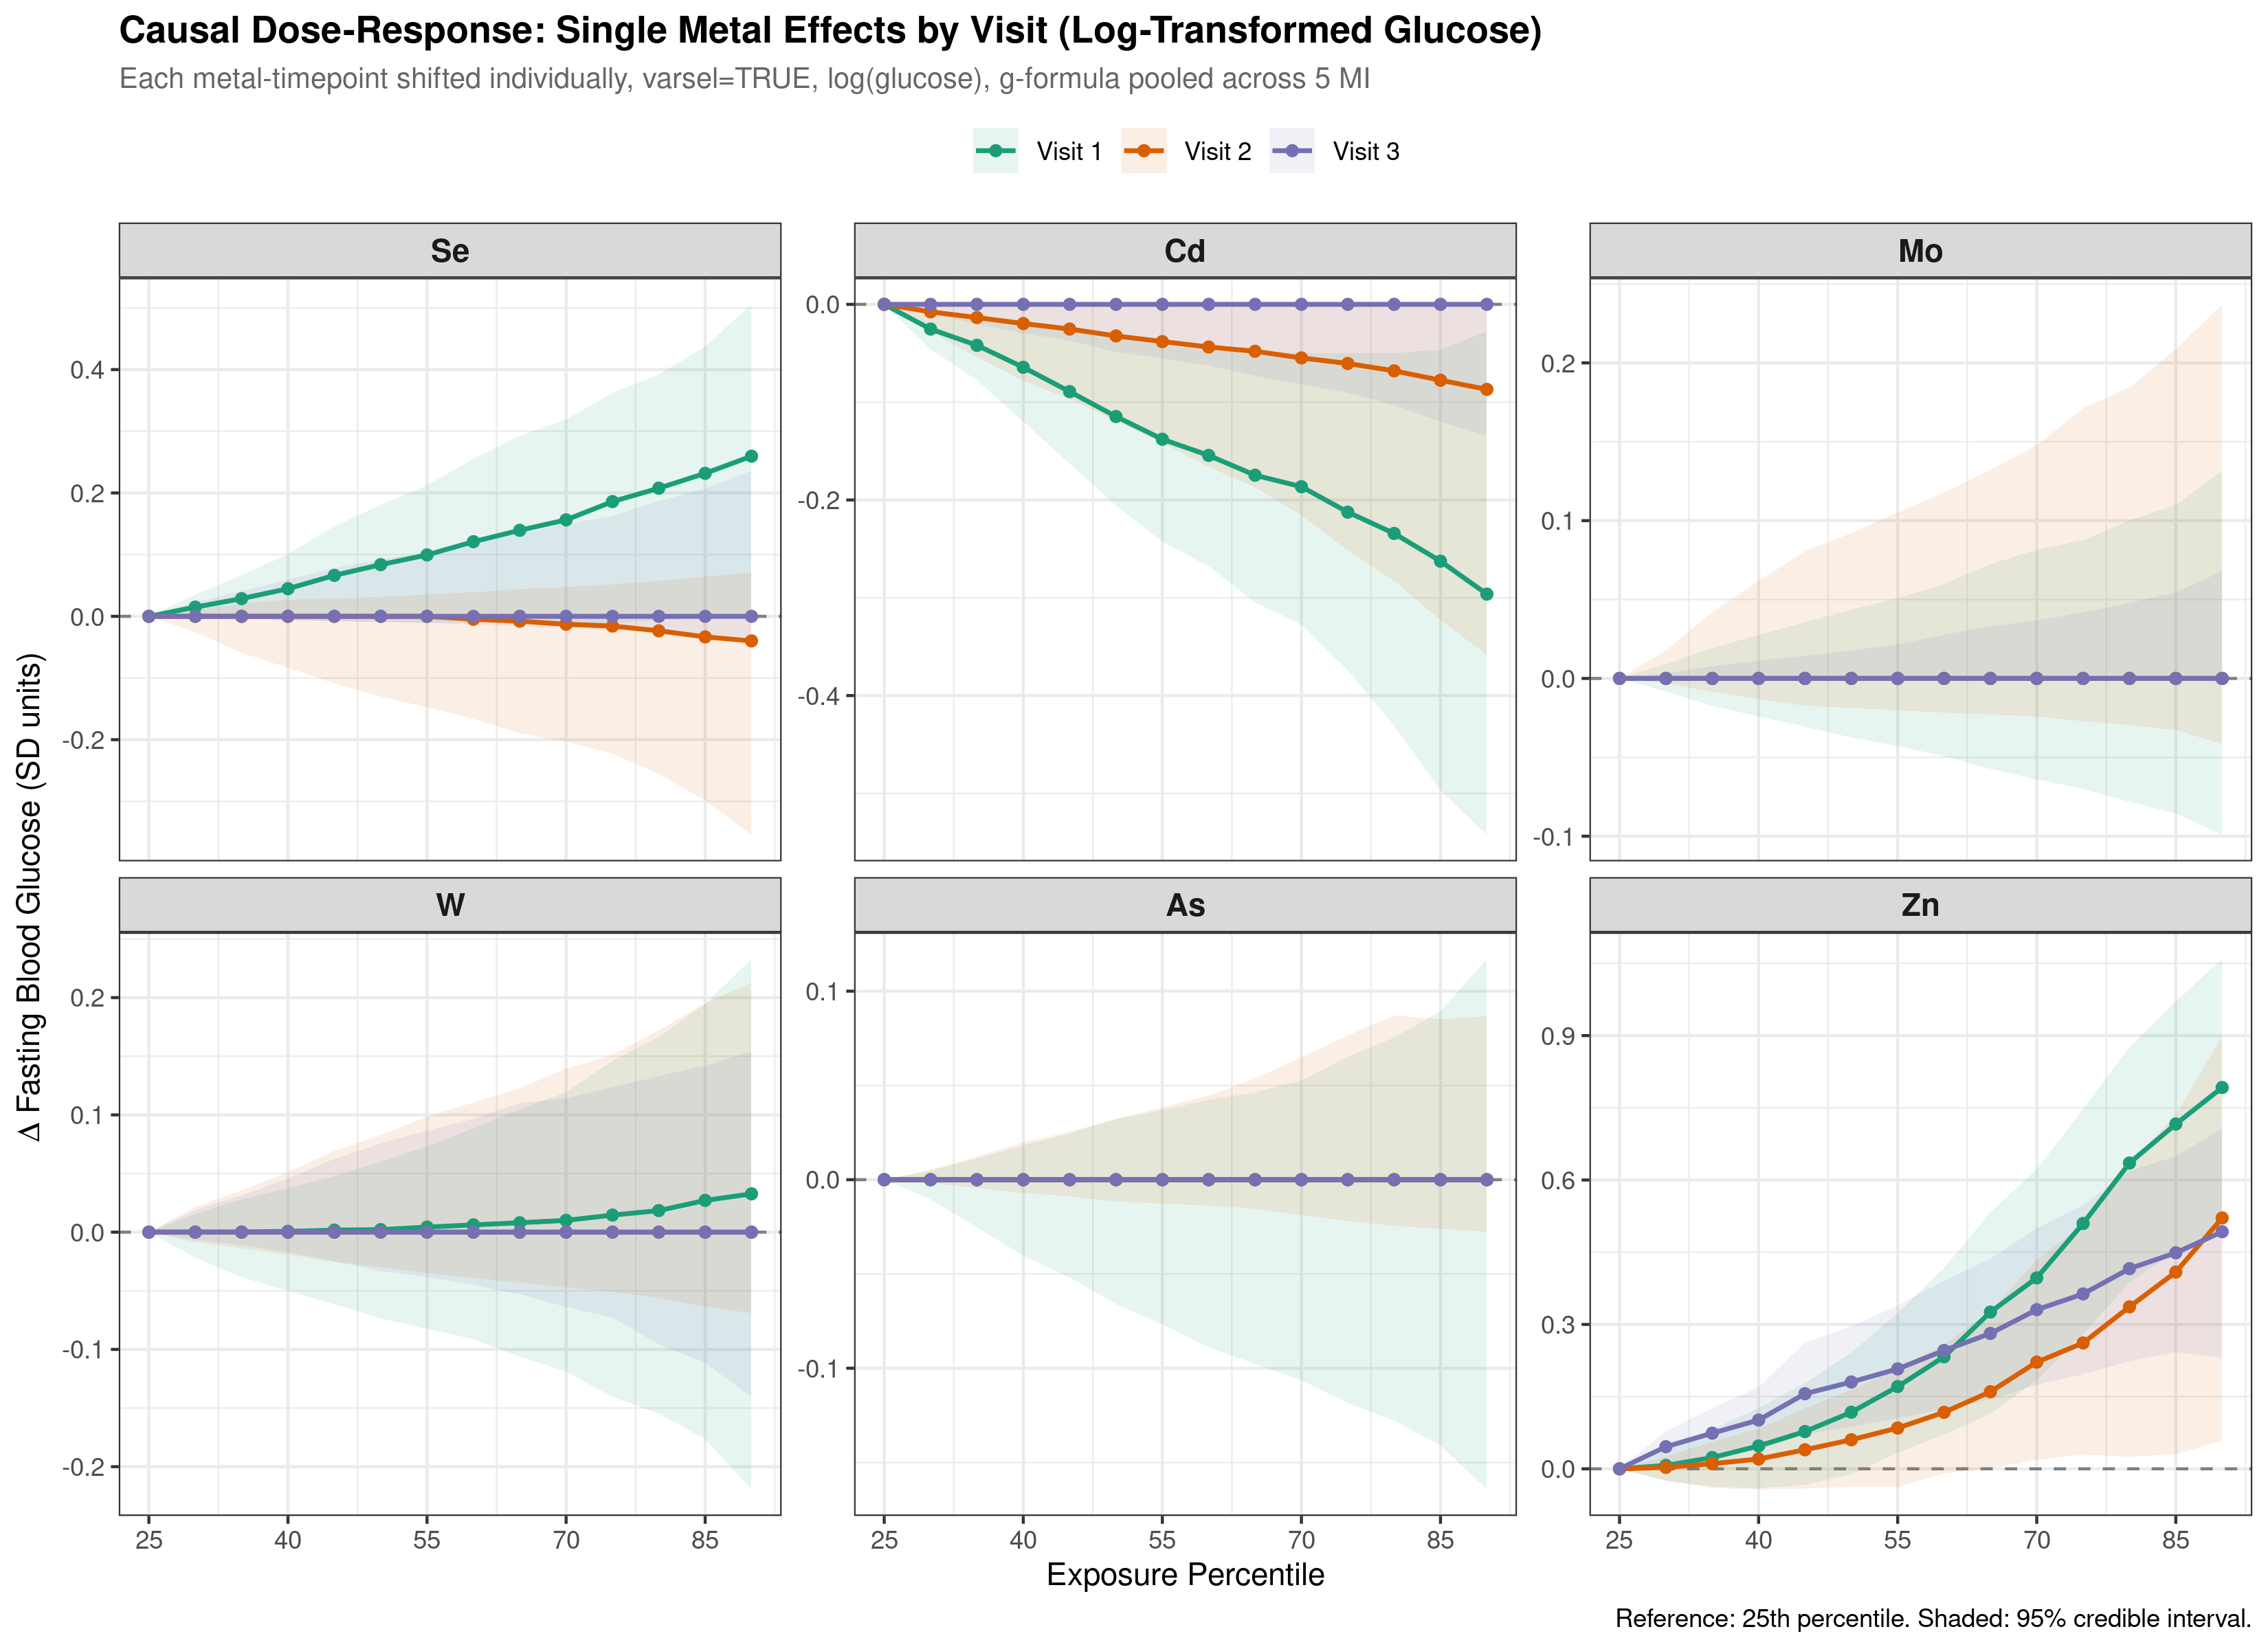
\includegraphics[width=0.85\textwidth]{figures/fig_permetal_full.png}
\caption{Per-metal dose-response curves (full sample, $n = 679$). Each panel: one metal shifted across percentiles, remaining exposures at the 50th percentile. Lines distinguish the three visits.}
\end{figure}

% ---- S2: Forest no-DM ----
\begin{figure}[h]
\centering
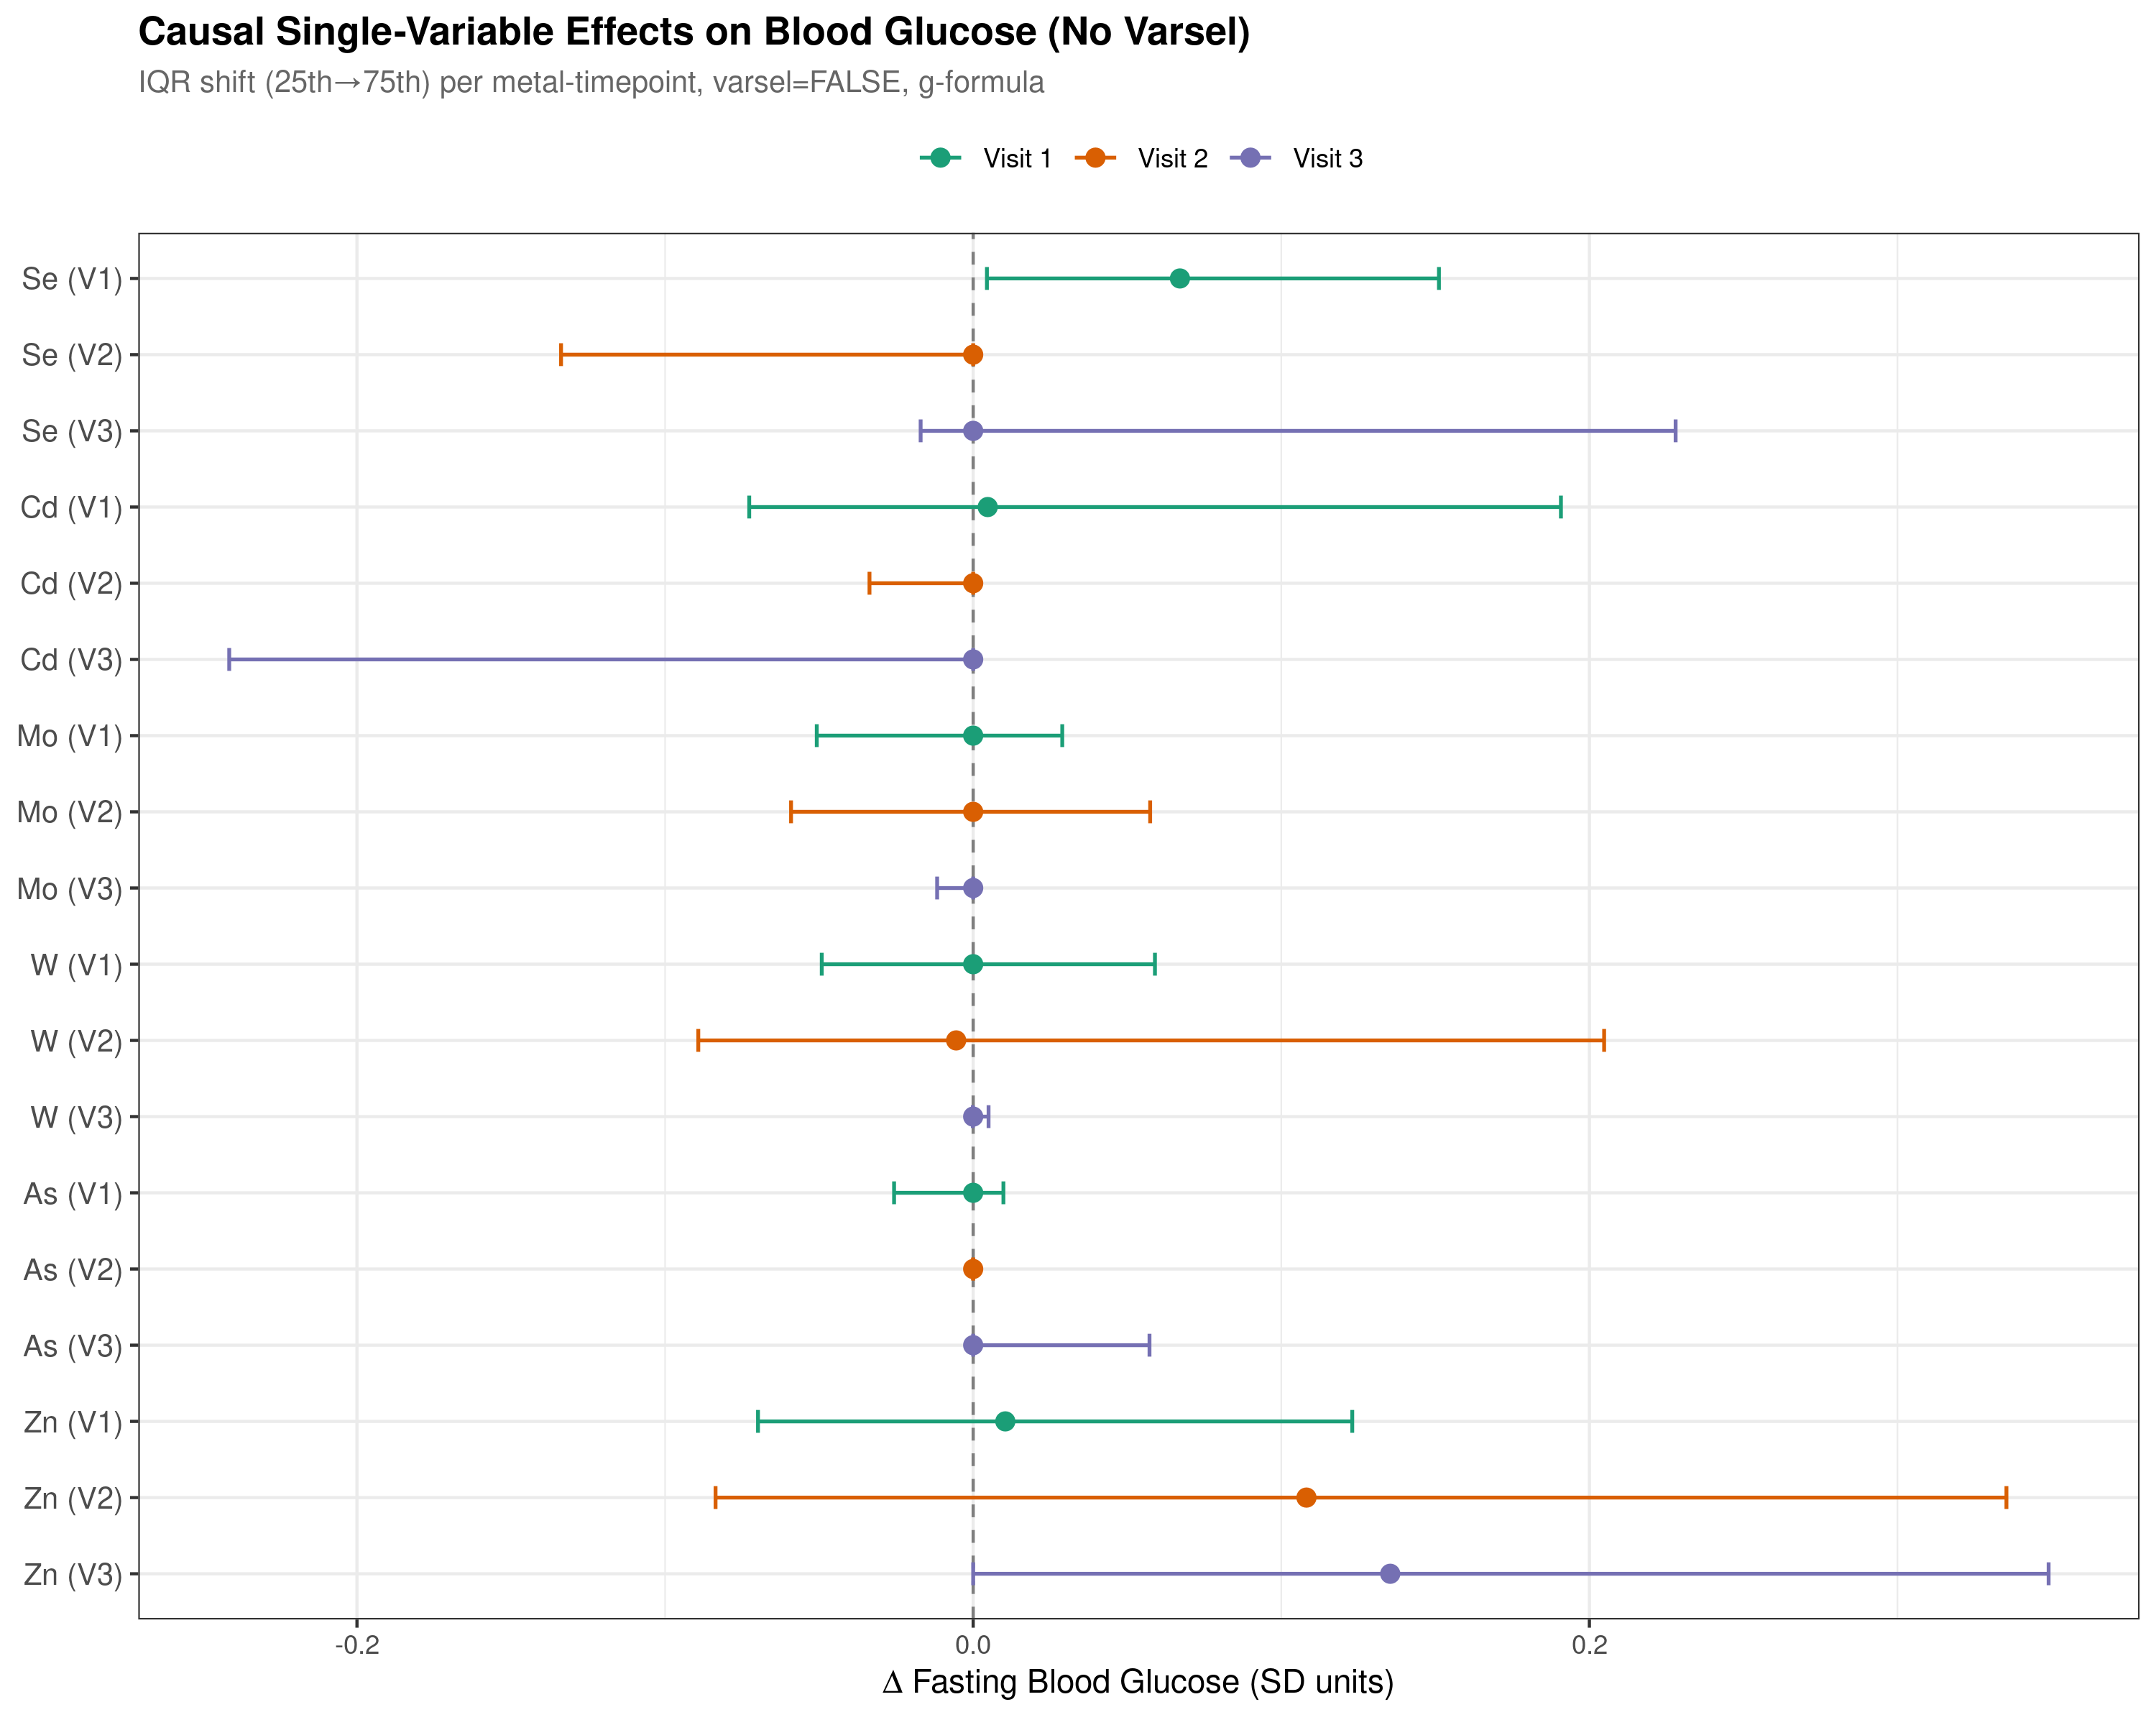
\includegraphics[width=0.85\textwidth]{figures/fig_forest_nodm.png}
\caption{Single-variable causal effects, excluding baseline diabetes ($n = 414$).}
\end{figure}

% ---- S3: Per-metal dose-response (no-DM) ----
\begin{figure}[h]
\centering
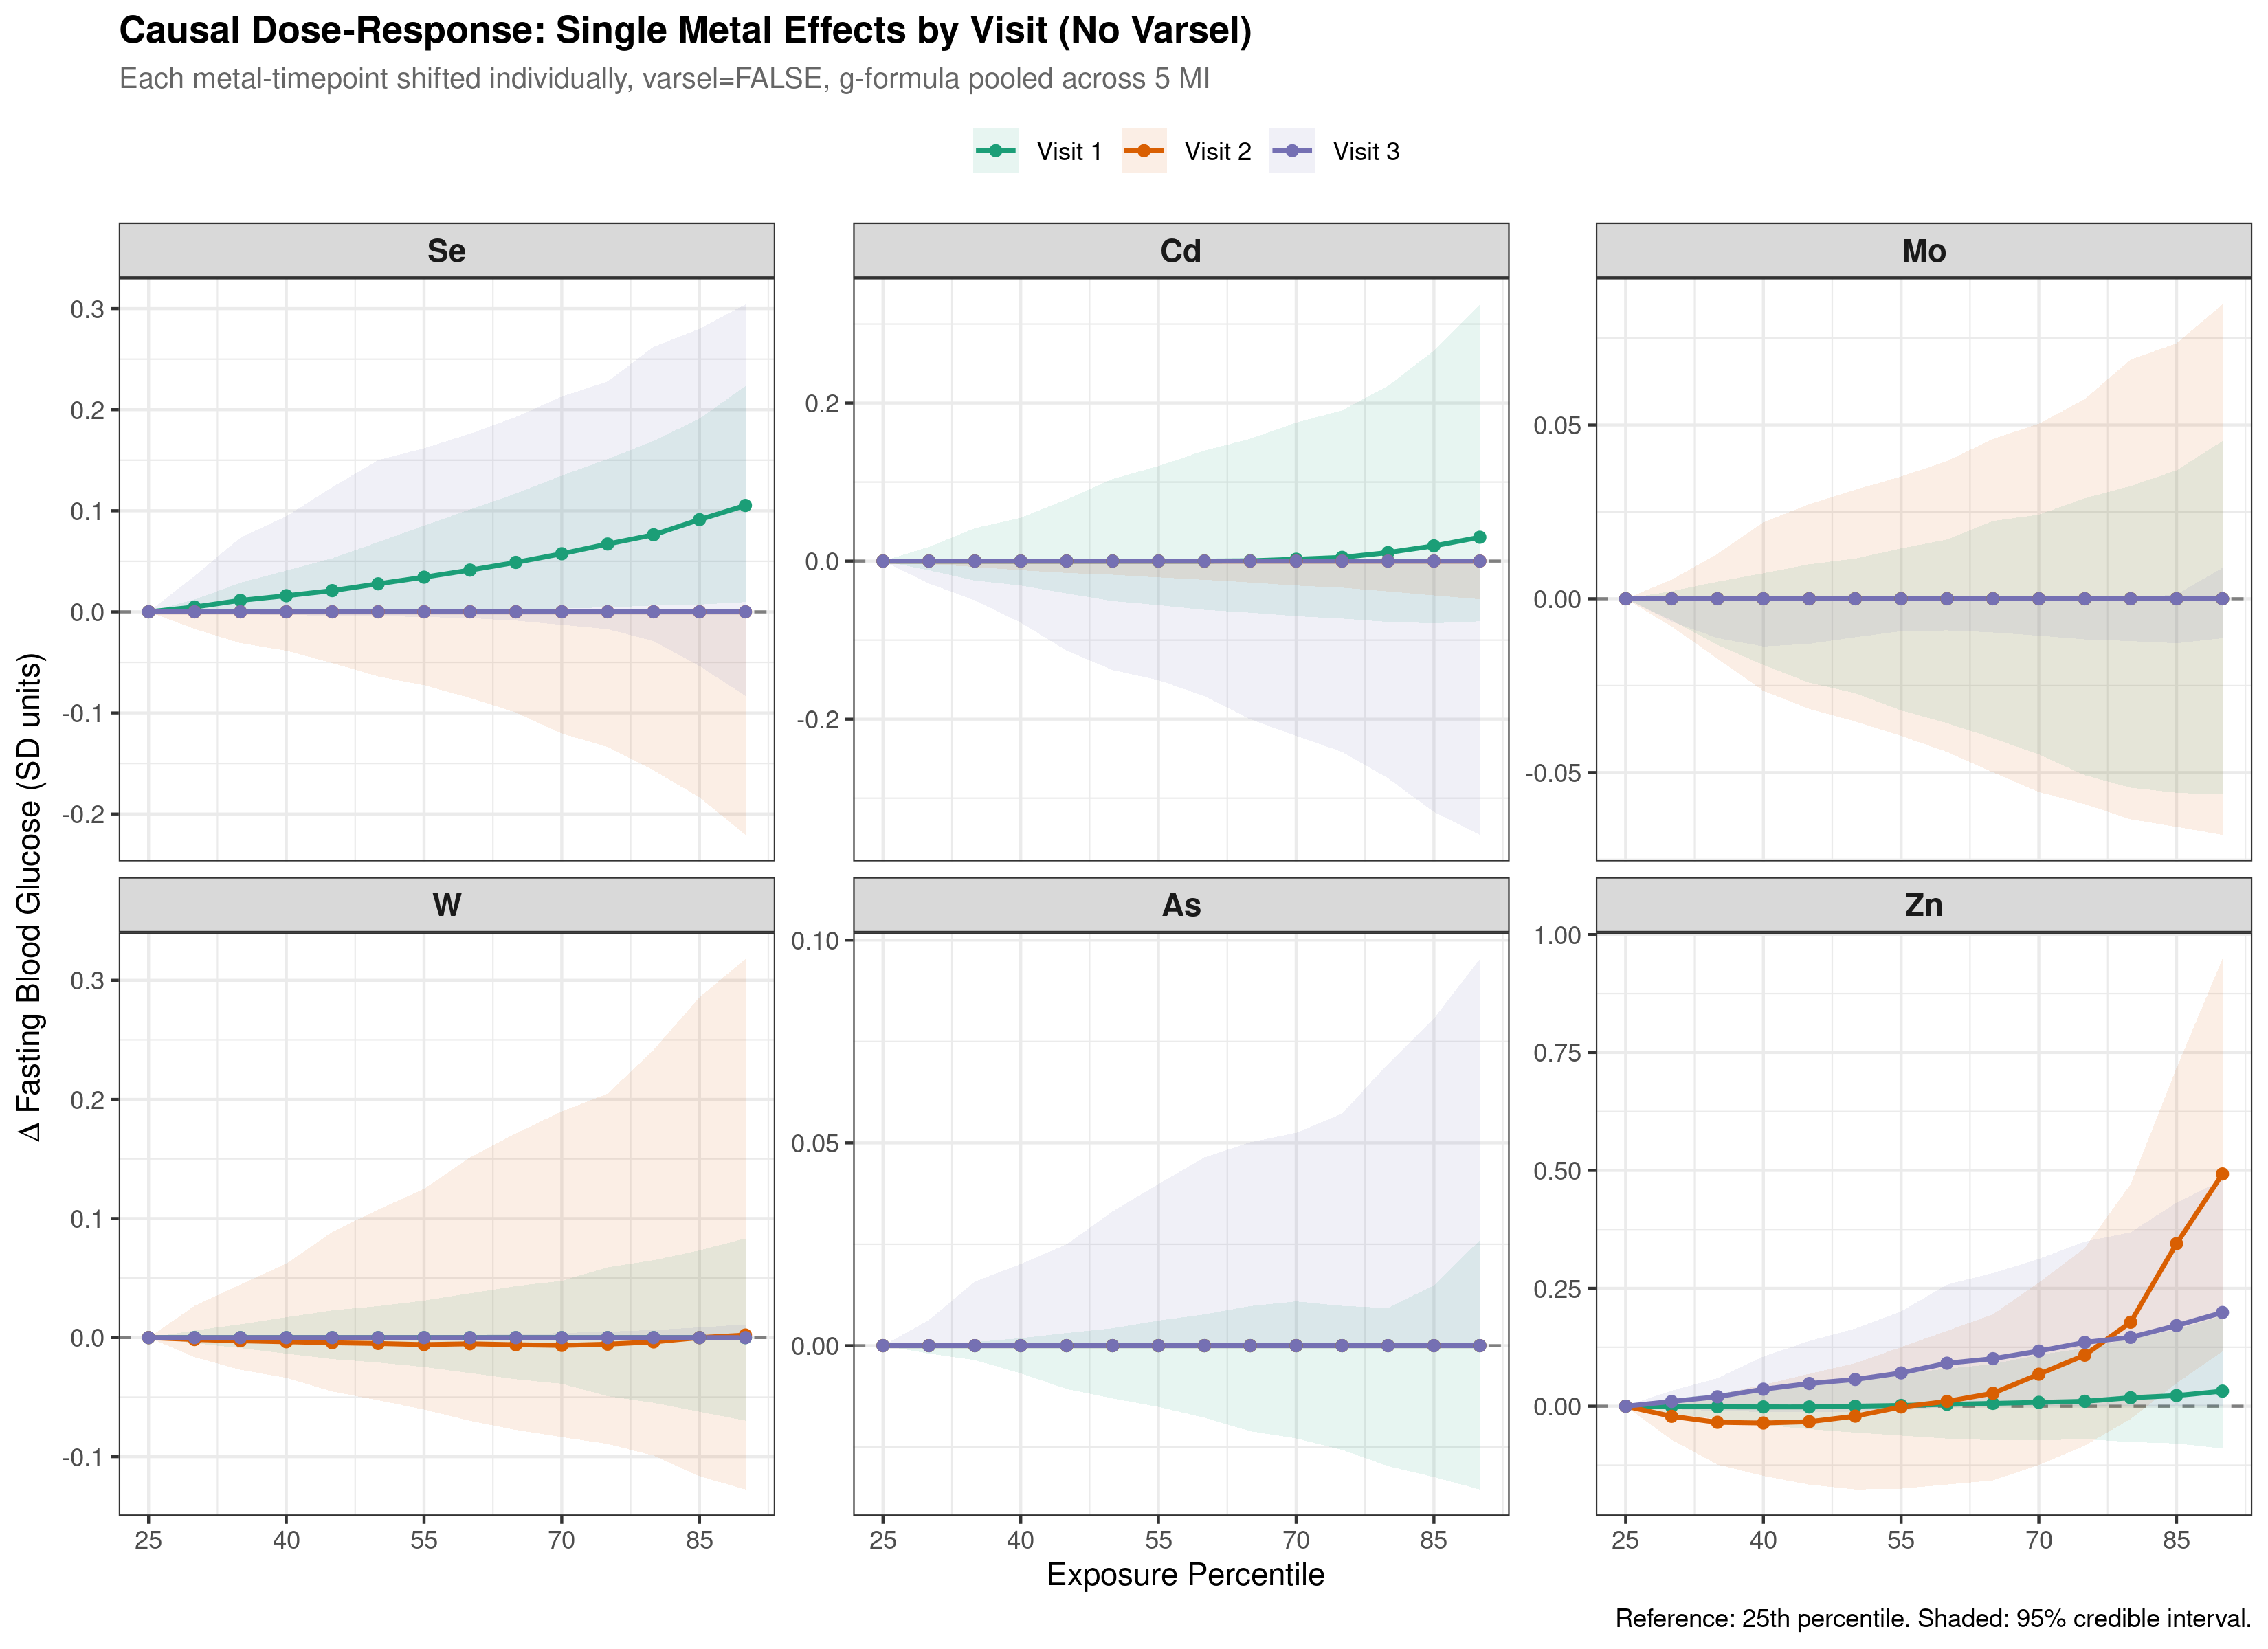
\includegraphics[width=0.85\textwidth]{figures/fig_permetal_nodm.png}
\caption{Per-metal dose-response curves, excluding baseline diabetes ($n = 414$).}
\end{figure}

% ---- S4: Dose-response pack-years ----
\begin{figure}[h]
\centering
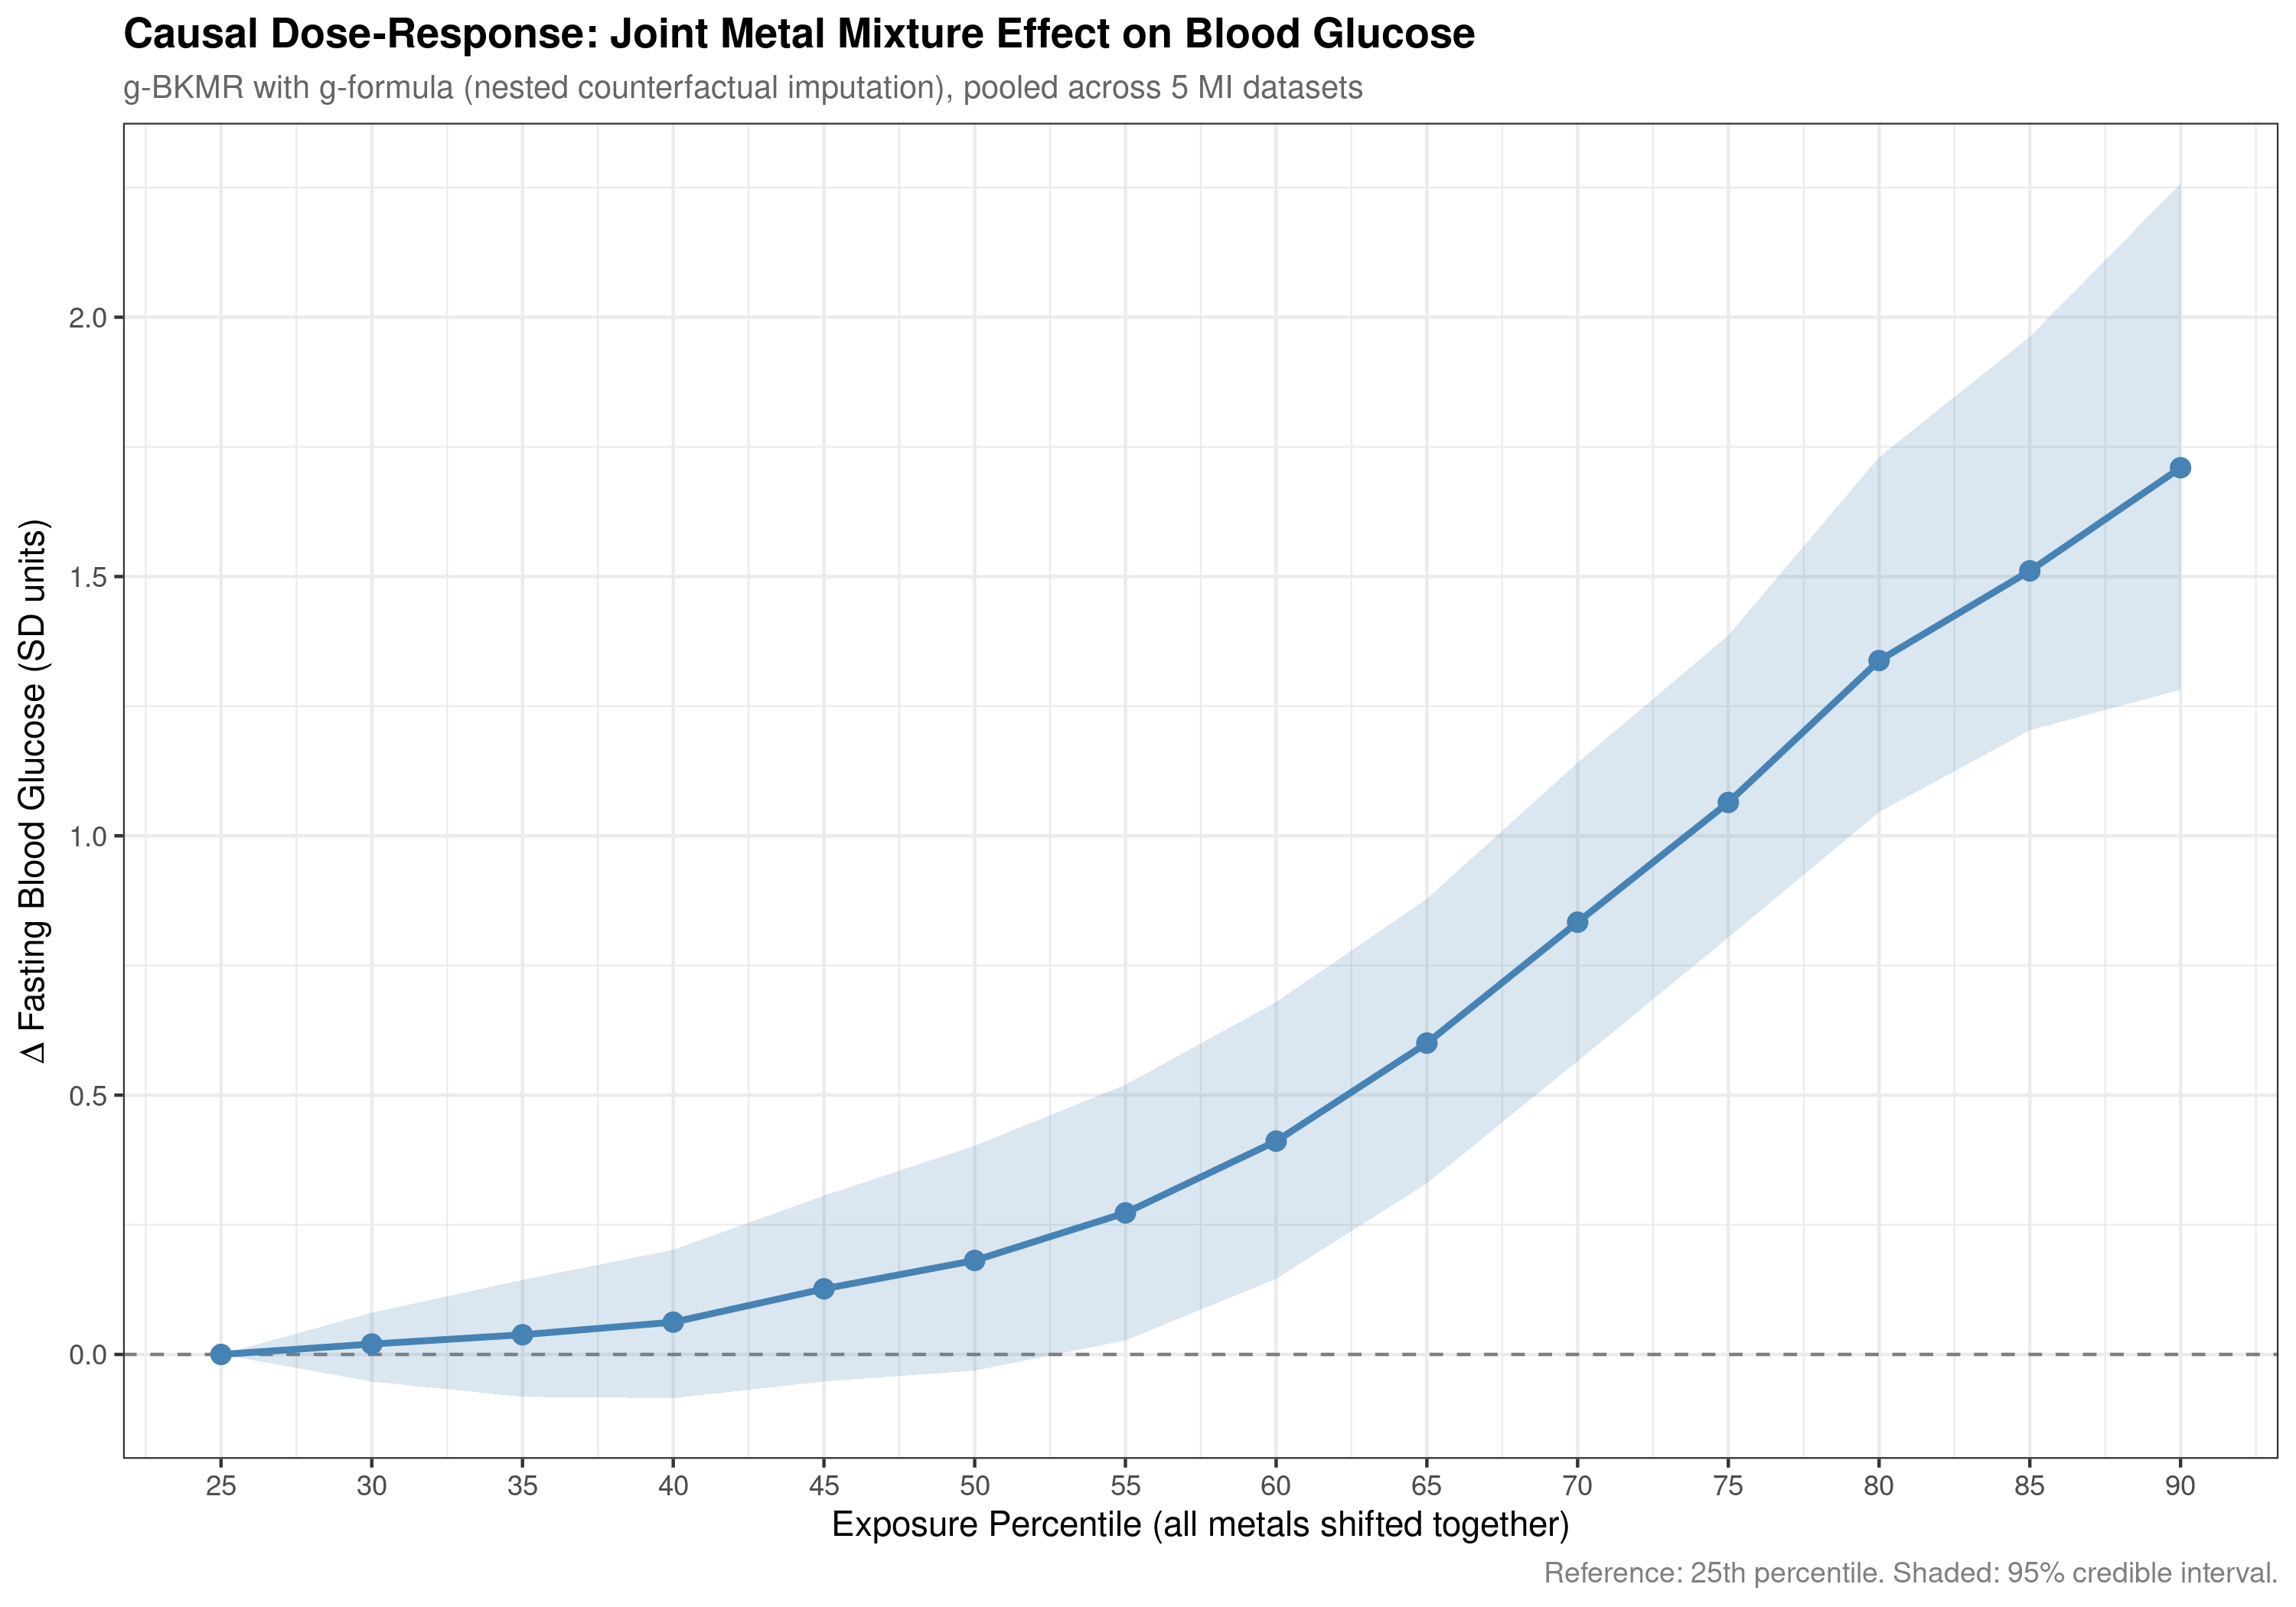
\includegraphics[width=0.85\textwidth]{figures/fig_dr_packyears.png}
\caption{Sensitivity: joint dose-response after additionally adjusting for baseline pack-years ($n = 679$).}
\end{figure}

% ---- S5: Forest pack-years ----
\begin{figure}[h]
\centering
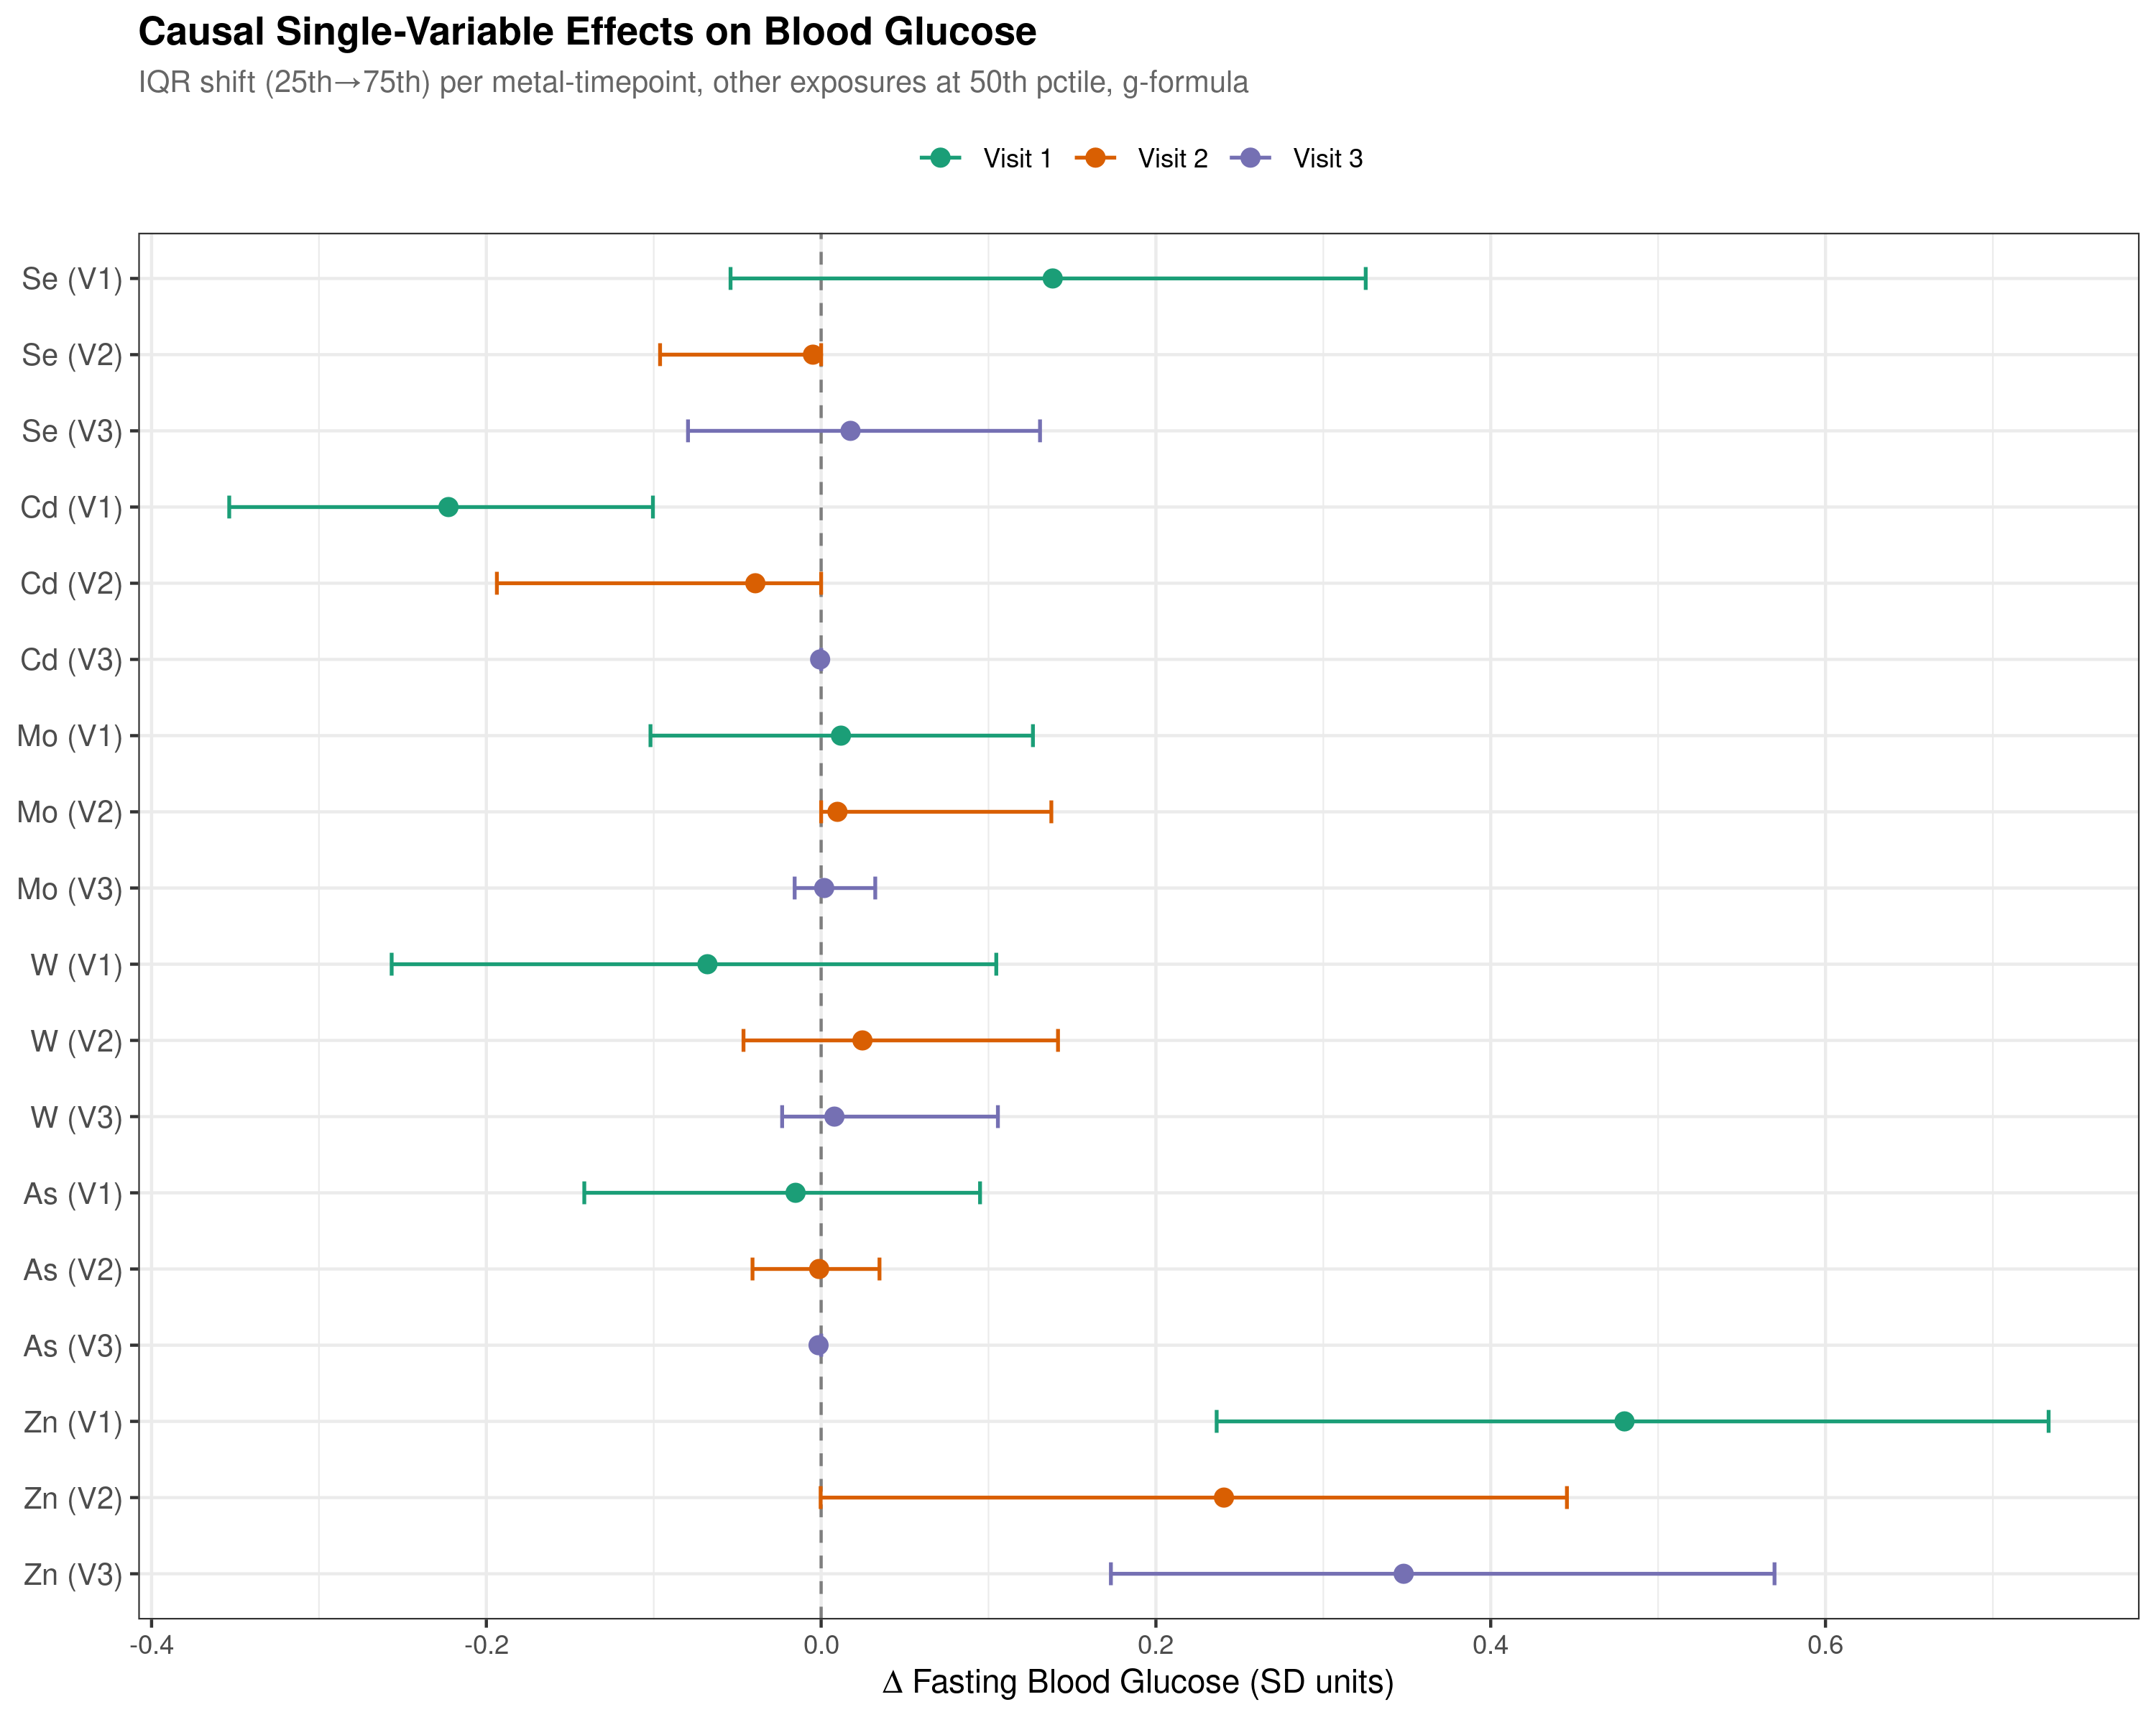
\includegraphics[width=0.85\textwidth]{figures/fig_forest_packyears.png}
\caption{Sensitivity: single-variable causal effects after additionally adjusting for baseline pack-years ($n = 679$).}
\end{figure}

% ---- S6: Per-metal dose-response pack-years ----
\begin{figure}[h]
\centering
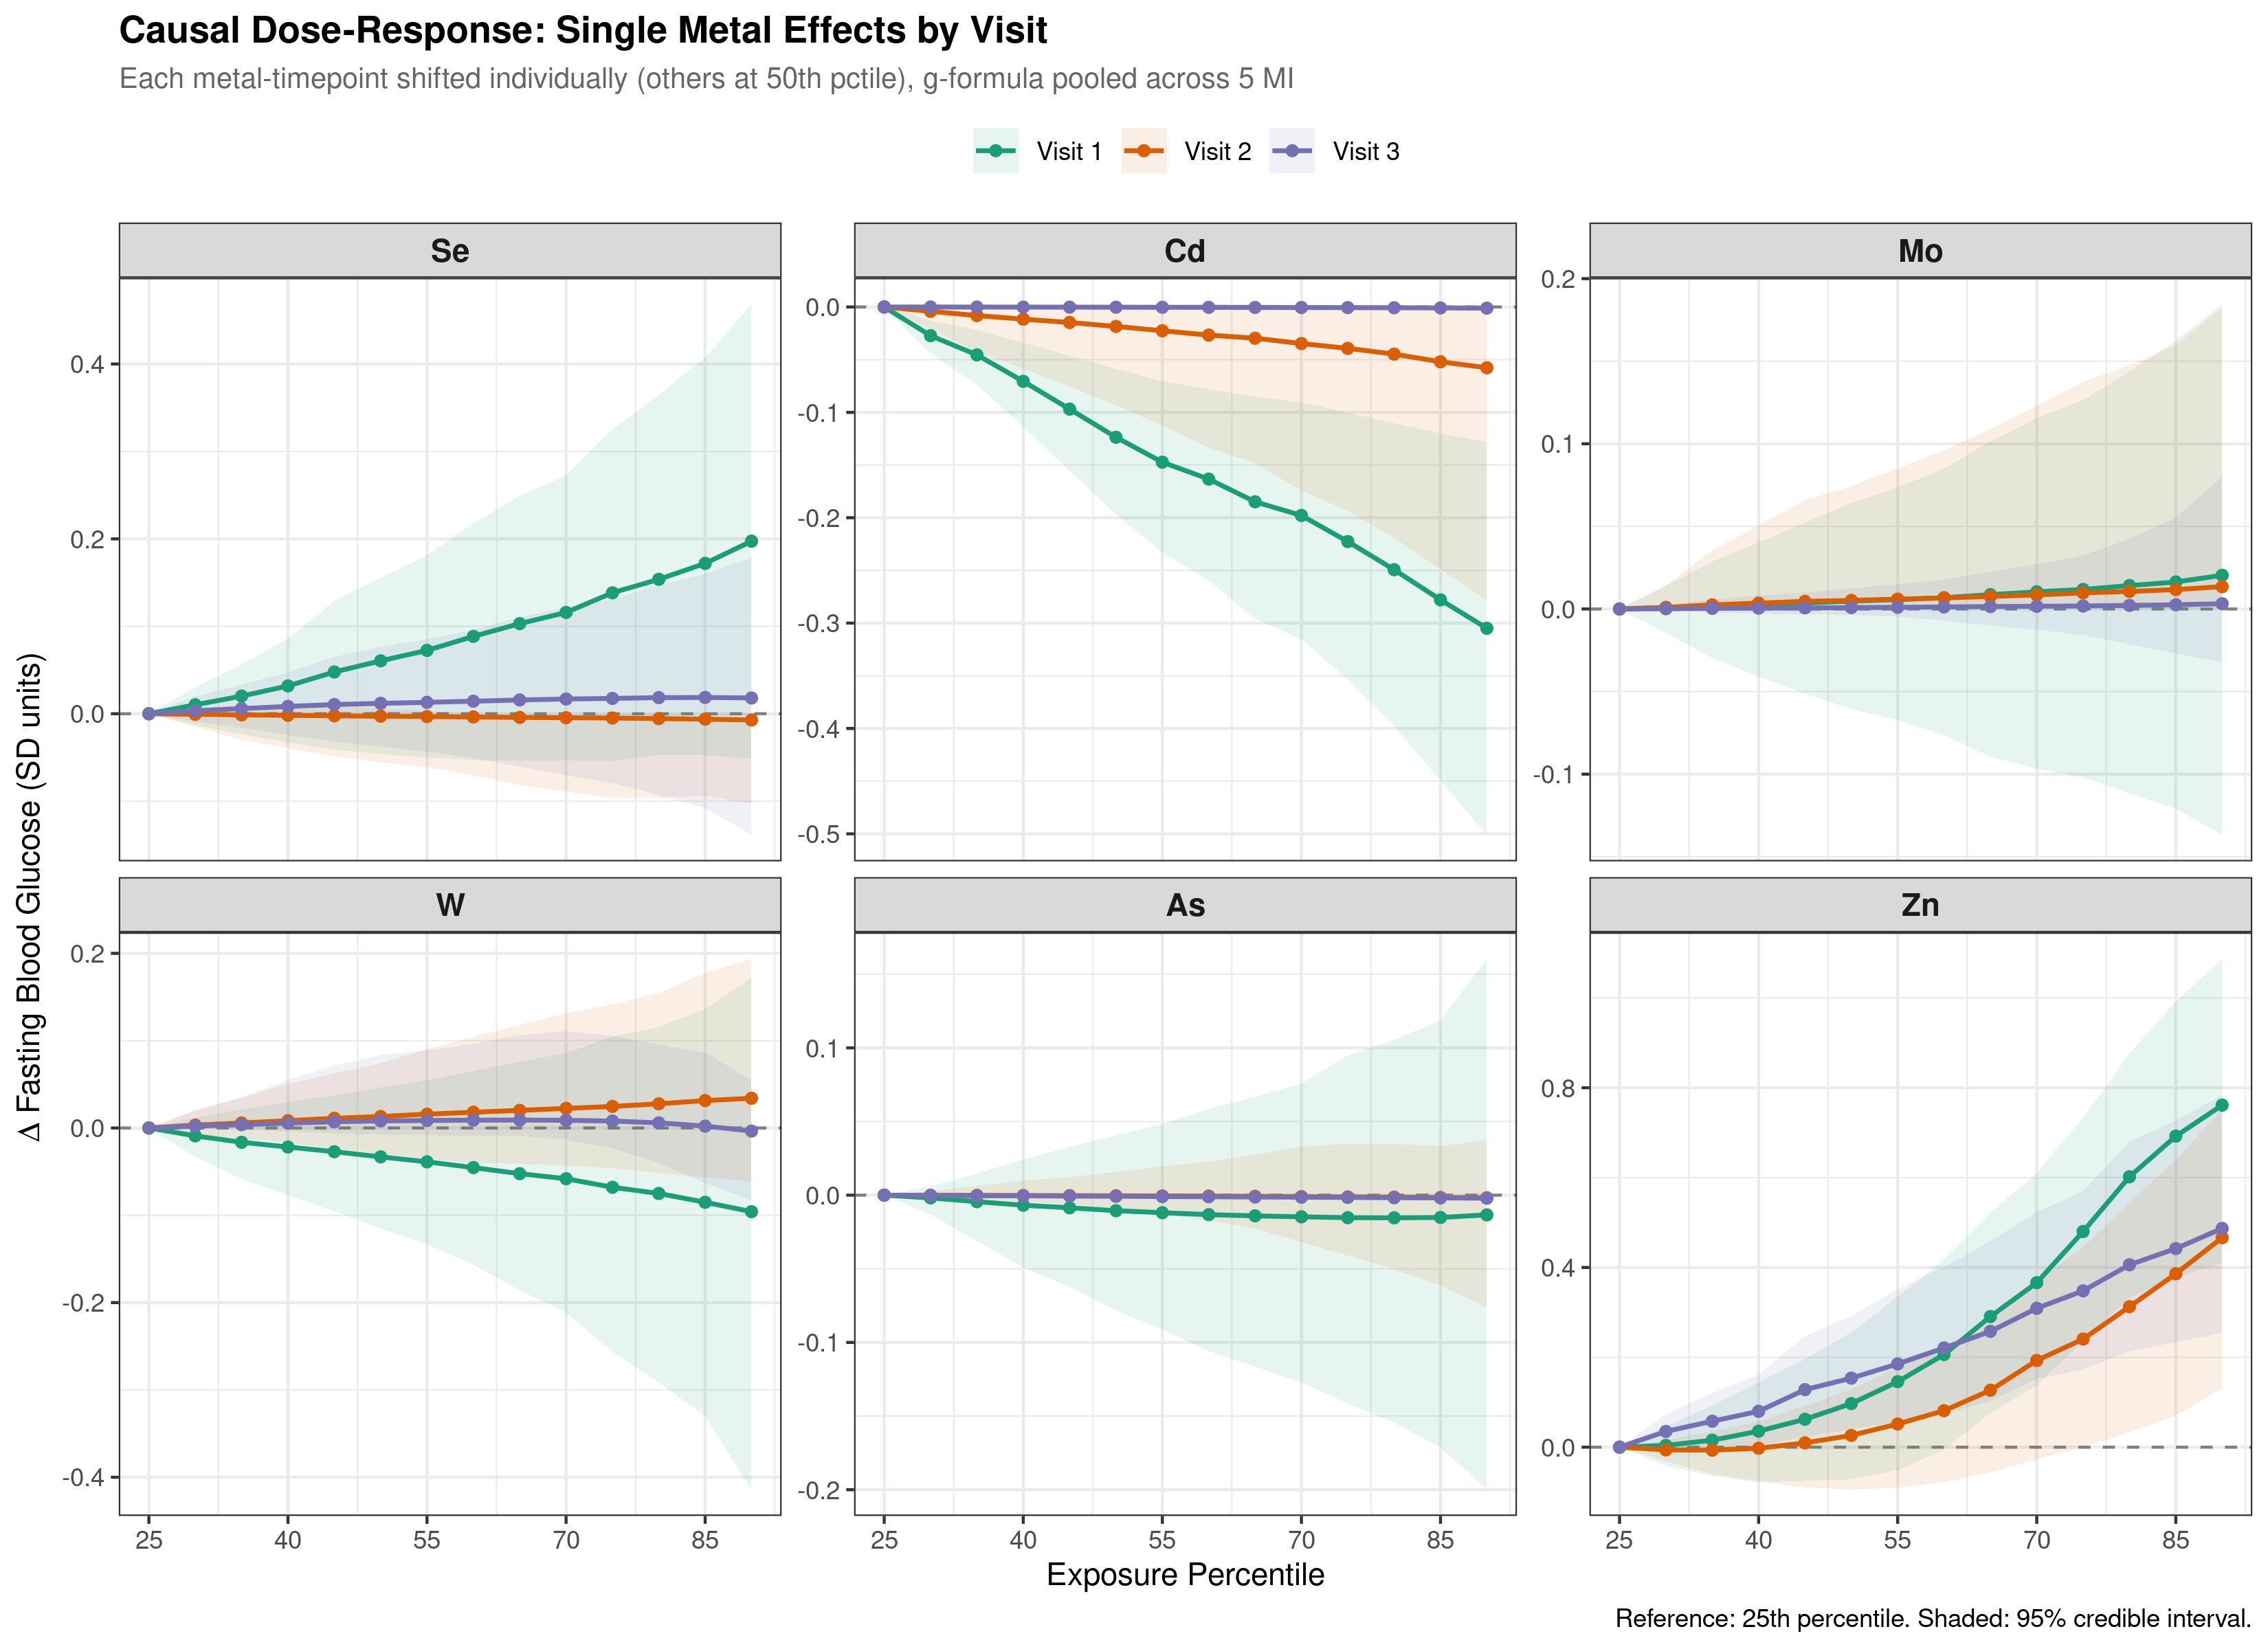
\includegraphics[width=0.85\textwidth]{figures/fig_permetal_packyears.png}
\caption{Sensitivity: per-metal dose-response curves after additionally adjusting for baseline pack-years ($n = 679$).}
\end{figure}

% ---- S7: MCMC trace plots ----
\begin{figure}[h]
\centering
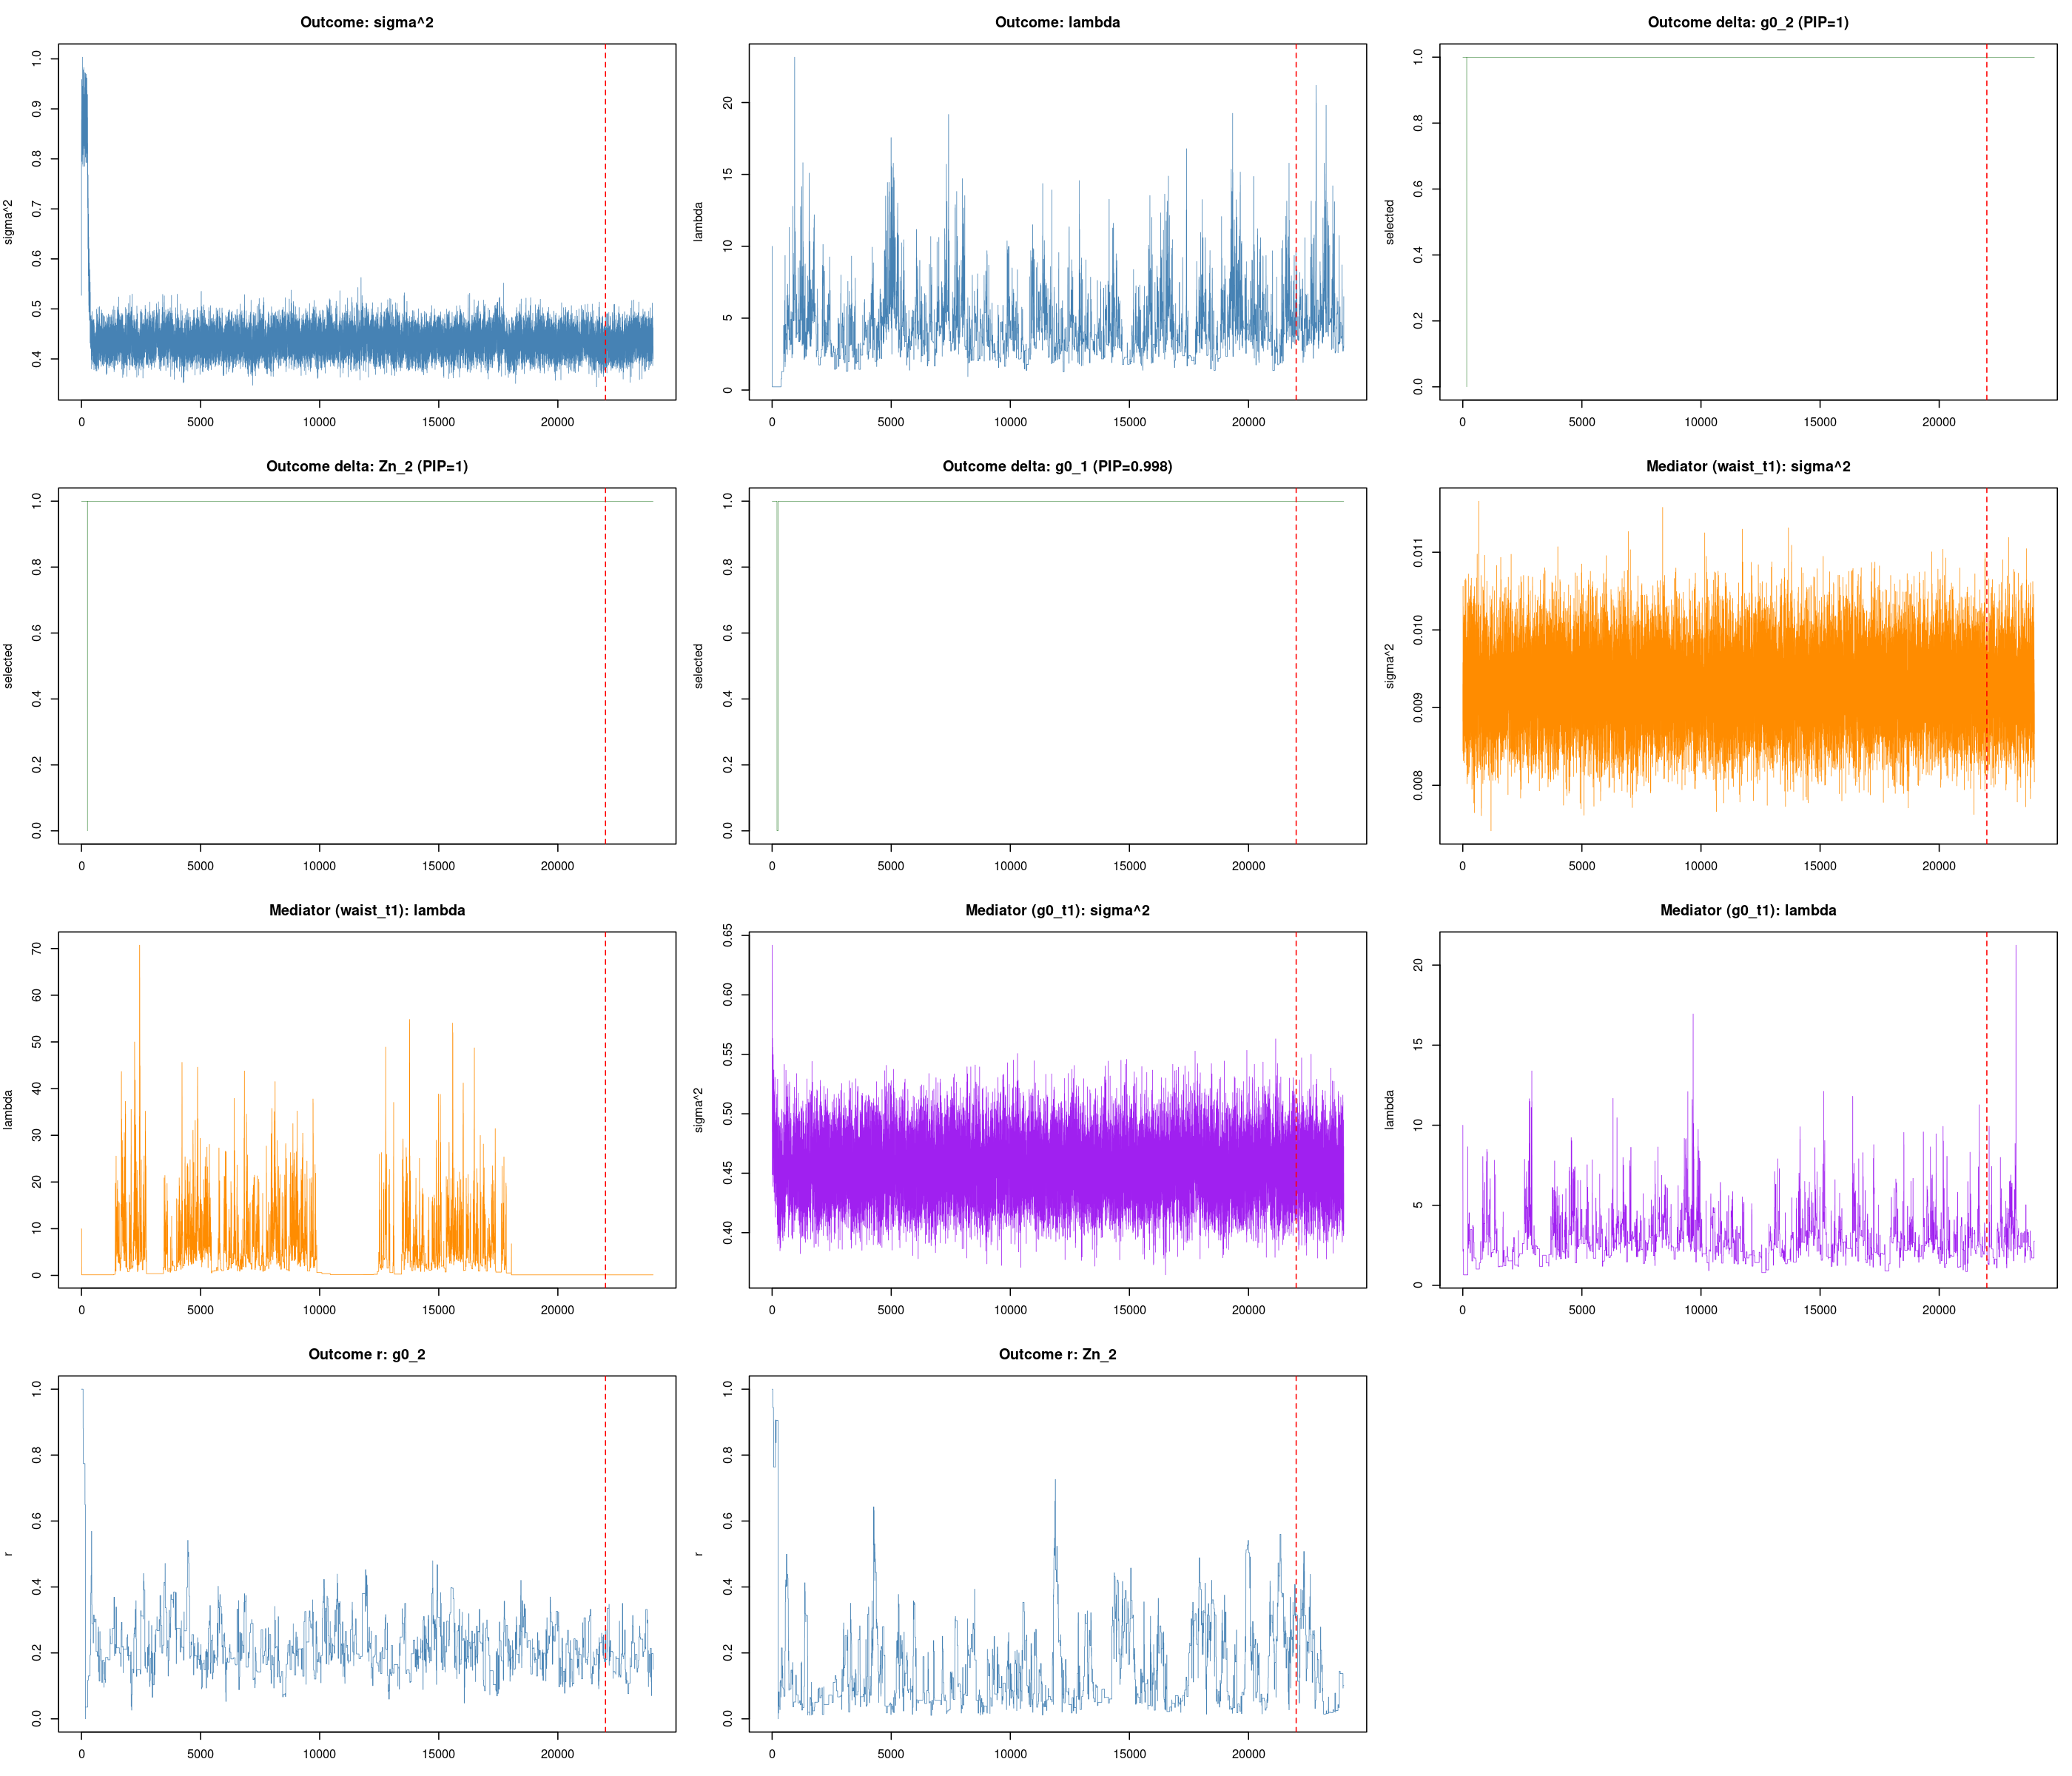
\includegraphics[width=0.9\textwidth]{figures/fig_traceplots.png}
\caption{MCMC trace plots for representative BKMR models in the main analysis. Chains showed good mixing, rapid transit between regions of the posterior, and no drift, indicating appropriate convergence for the retained posterior window (iterations $22{,}000$--$24{,}000$).}
\end{figure}
